% Article type supporting font formatting
\documentclass[a4paper,12pt]{extarticle}

% Define .tex file encoding
\usepackage[utf8]{inputenc}

% Norwegian language support
%\usepackage[norsk]{babel}     

% Indent first paragraph in section
\usepackage{indentfirst}

% Allows mathbb in tex file
\usepackage{amsfonts} 

% Margin defining package
\usepackage{geometry}         
\geometry{a4paper
  ,margin=2cm
}

% Allows easy writing of algorithms
\usepackage[ruled]{algorithm2e}

% Math related tools and functions
\usepackage{mathtools} 

% For quotations
\usepackage{csquotes}

% Better bibliography 
\usepackage[round]{natbib}

% For use of graphics in document
\usepackage{graphicx}         

% Allows multi-line comments in tex file
\usepackage{verbatim} 

% Allows more control over tables
\usepackage{tabulary}

% Ads ul which allows line breaks while underlining text.
\usepackage{soul}      

% Allows math in tex file 
\usepackage{amsmath}          

% Allows math symbols in tex file
\usepackage{amssymb}          

% Allows use of physics shortcut functions
%\usepackage{physics}          

% Verbatim env with LaTeX commands
\usepackage{alltt}            

% Allows \begin{figure}[H]
\usepackage{float}

% Adds labeling list to the report
\usepackage{scrextend}
\addtokomafont{labelinglabel}{\ttfamily}

% Necessary for defining colours
\usepackage{xcolor}            
\definecolor{linkgreen}{rgb}{0,.5,0}
\definecolor{linkblue}{rgb}{0,0,.5}
\definecolor{linkred}{rgb}{.5,0,0}
\definecolor{blue}{rgb}{.13,.13,1}
\definecolor{green}{rgb}{0,.5,0}
\definecolor{red}{rgb}{.9,0,0}

% Hyperlinks in document
\usepackage{hyperref}  
\hypersetup{
  colorlinks=true,     % True for colored links
  linktoc=all,         % True for table of contents links
  linkcolor=linkblue,  % Colour for links
  urlcolor=linkgreen,  % Colour for URLs
  citecolor=linkred    % Colour for citations
}

% Listing package for code examples
\usepackage{listings}         
\lstset{
  language=C++,                % Set language to C++
  showspaces=false,            % Don't show space chars
  showtabs=false,              % Don't show tab chars
  breaklines=true,             % Break long lines of code
  showstringspaces=false,      % Don't show spaces in strings
  breakatwhitespace=true,      % Break at white space only
  commentstyle=\color{green},  % Set colour for comments
  keywordstyle=\color{blue},   % Set colours for keywords
  stringstyle=\color{red},     % Set colour for strings
  basicstyle=\ttfamily,        % Set basic style
  tabsize=2                    % Set tabsize
}

% Makes matrices look square-ish
\renewcommand*{\arraystretch}{1.5}

% Allows number referencing the last page, used in footer
\usepackage{lastpage}

% Allows editing of header and footer data
\usepackage{fancyhdr}
\fancypagestyle{plain}{
  \fancyhf{}
  \renewcommand{\headrulewidth}{0pt}
  \rfoot[R]{\footnotesize Page \thepage\ of \pageref{LastPage}}
}
\pagestyle{fancy}
\fancyhf{}
\chead{\footnotesize D.A. Salwerowicz, From B-Spline to GERBS Curve and Surface, affine transformations as special effects}
\rfoot{\footnotesize Page \thepage\ of \pageref{LastPage}}
\setlength{\headheight}{20pt}
\setlength{\footskip}{20pt}

% Allows editing of section headers
\usepackage{titlesec}
\titleformat*{\section}{\normalsize\bfseries}
\titleformat*{\subsection}{\normalsize\itshape\bfseries}
\titleformat*{\subsubsection}{\normalsize\bfseries}

% Change look and feel of abstract
\usepackage{abstract}
\setlength{\absleftindent}{0mm}
\setlength{\absrightindent}{0mm}
\renewcommand*\abstractname{\flushleft\normalsize\textbf{Abstract}\hfill}

% Change caption size and style
\usepackage[font=footnotesize,labelsep=period]{caption}

% Change date style
\usepackage[yyyymmdd]{datetime}
\renewcommand{\dateseparator}{-}

% Referencing, last for compatibility reasons
\usepackage[noabbrev]{cleveref}

%%%%%%%%%%%%%%%%%%%%%%%%%%%%%%%%%%%%%%%
%%      Title, Author, and Date      %%
%%%%%%%%%%%%%%%%%%%%%%%%%%%%%%%%%%%%%%%
\title{From B-Spline to GERBS Curve and Surface, affine transformations as special effects}
\author{D. A. Salwerowicz (dsa014)}
\date{\parbox{\linewidth}{\centering
    \textit{\small UiT - The Arctic University of Norway, P.O. Box 385, N-8505 Narvik, Norway}\endgraf\bigskip
    \small Submitted \today
}}
\providecommand{\keywords}[1]{\flushleft\textit{\small{Keywords:}} #1}

%%%%%%%%%%%%%%%%%%%%%%%%%%%%%%%%%%%%%%%
%%           Start document          %%
%%%%%%%%%%%%%%%%%%%%%%%%%%%%%%%%%%%%%%%
\begin{document}
  
%%%%%%%%%%%%%%%%%%%%%%%%%%%%%%%%%%%%%%%
%%   Create the main title section   %%
%%%%%%%%%%%%%%%%%%%%%%%%%%%%%%%%%%%%%%%
\maketitle

%%%%%%%%%%%%%%%%%%%%%%%%%%%%%%%%%%%%%%%
%%      Abstract for the report      %%
%%%%%%%%%%%%%%%%%%%%%%%%%%%%%%%%%%%%%%%
\noindent\rule{\linewidth}{.5pt}
\begin{abstract} 
The project I worked revolved around implementing GERBS Curves and Surfaces as well as animating them using affine transformations. This report describes necessary theory for understanding GERBS curves and surfaces as well as how they were implemented in GMlib and C++.

\keywords{Parametric Curves; B-Splines; Curve Blending; GERBS}
\end{abstract}
\rule{\linewidth}{.5pt}

%%%%%%%%%%%%%%%%%%%%%%%%%%%%%%%%%%%%%%
%%  The main content of the report  %%
%%%%%%%%%%%%%%%%%%%%%%%%%%%%%%%%%%%%%%

\section{Introduction}
This project revolved around implementing various geometric objects using GMlib as a basis. Each of these object builds on previous, therefore I will describe them in order, from least to most complex. Main focus of this project was to implement a GERBS curve and use affine transformations to create a dynamic animation.

\subsection{B-Spline curve}
Most basic object that I have implemented is a third degree, fourth order B-Spline curve using both a vector of \emph{control points} and \emph{least square approximation}.

\subsection{Blending curve}
A more advanced object I implemented was a blending curve that takes in two curves and blends them into one curve using any percent of the original curves it wants. So I can use arbitrary percentage of these curves and blend the rest.

\subsection{GERBS curves and surfaces}
Last and most complex implemented objects were GERBS curves and surfaces, where GERBS stands for \emph{Generalized Expo-Rational B-Spline}. These objects use local curves and surfaces that are blended together to form a curve/surface, instead of control points.

\section{Material \& Methods}
This section describes the most important tools and methods used during development of my project. Most of the theory in this section is based on book "Blending technics[sic] for Curve and Surface Constructions" written by Arne Laks\aa \,\citep{Laksa2012}, and his lectures in class.

\subsection{GMlib}
It's important to mention that I have based my project work on the \emph{Geometric Modeling library} also known as GMlib. It was developed at Arctic University of Norway, UiT Narvik. It handles a lot of necessary background calculation and rendering of objects on screen for me. This way I only needed to focus on implementing necessary functionality and calculations for showing B-Spline curves and other objects.

\subsection{B-Spline Curves}
\subsubsection{B-Spline from control points}
One can create a B-Spline curve from a vector of \emph{control points} $\vec{c}$, which is then used to create a \emph{knot vector} $\vec{t}$. For any given B-Spline a knot vector will be of length $n+k$ where $n$ is length of control point vector and $k$ is the order. So for my 3\textsuperscript{rd} degree B-Spline knot vector will have lenght 12 if I give it 8 control points. Resulting knot vector will look like one shown in \cref{eq:KnotVectorBSpline}.

\begin{equation}
\vec{t}= [0,0,0,0,1,2,3,4,5,5,5,5]
\label{eq:KnotVectorBSpline}
\end{equation}

This B-Spline will be a \emph{Clamped B-Spline} as its first $k$ and last $k$ knots are equal to each other. Then I can use formula \cref{eq:BSplineFormula} to calculate my B-Spline.

\begin{equation}
c(t)= \sum_{i=1}^{n} c_i b_{k,i}(t), \quad t \in \left[t_d,t_n\right]
\label{eq:BSplineFormula}
\end{equation}

Here ${c_i}_{i=1}^n$ is a vector of controll point and $b_{k,i}(t)$ are basis functions that are defined by $t$ \citep[Chap 5.5.1]{Laksa2012}. \citep[Chap 5.5.3]{Laksa2012} describes in depth how we calculate these basis functions. Resulting basis functions are shown in \cref{eq:BasisFunctions}, there are four of them, since the order of my B-Spline is $4$.

\begin{equation}
\begin{split}
b_{k-3,i} &= \left[ \left( 1-w_{1,i}(t) \right) \left( 1-w_{2,i-1}(t) \right) \right] \left[ 1-w_{3,i-2}(t) \right]\\
b_{k-2,i} &= \left[ \left( 1-w_{1,i}(t) \right) \left( 1-w_{2,i-1}(t) \right) \right] \left[ 1-w_{3,i-1}(t) \right]\\ &+ \left( \left[ \left( 1-w_{1,i}(t) \right) \left( w_{2,i-1}(t) \right) \right] + \left[ w_{1,i}(t) \left( 1-w_{2,i}(t) \right) \right] \right) \left[ 1-w_{3,i-t}(t) \right]\\
b_{k-1,i} &= \left( \left[ \left( 1-w_{1,i}(t) \right) \left( w_{2,i-1}(t) \right) \right] + \left[ w_{1,i}(t) \left( 1-w_{2,i}(t) \right) \right] \right) \left[ w_{3,i-1}(t) \right]\\
b_{k,i} &= w_{1,i}(t) w_{2,i}(t) w_{3,i}(t)
\label{eq:BasisFunctions}
\end{split}
\end{equation}

$w_{d,i}(t)$ is a so called linear translation and scaling function used in B-Splines to translate the $t$ to a range $[0,1]$, and is defined in \cref{eq:WFunction}.

\begin{equation}
  w_{d,i}(t) = 		
  \begin{cases}
    \frac{t-t_i}{t_{i+d} - t_i}, & \text{if } t_i \leq t \leq t_{i+d}\\
    0, & \text{otherwise.}
  \end{cases}
  \label{eq:WFunction}
\end{equation}

Thus using these basis functions I am able to evaluate my B-Spline and draw it on screen which is shown in the first simulation of my program.

\subsubsection{Sampled B-Spline}
Another way of creating a B-Spline is by sampling points along an existing curve and then using least square method to create control points from a set of sampled points $p$. It is quite usefull as it lets me approximate any kind of freeform curve to a high degree of accuracy.

Knot vector is created the same way as before, I just use the provided number of desired control points $n$ to create it. However in order to calculate $\vec{c}$ I have to perform matrix calculations. I start by calculating an $A$ matrix. Values in it are defined by formula in \cref{eq:LeastSquare}, which gives me a least square approximation of the original curve.

\begin{equation}
\partial t = \frac{t_n - t_d}{m-1}
\label{eq:LeastSquare}
\end{equation}

Where $m$ is the dimension of $p$. Algorithm used to calculate values in $A$ matrix is as shown in \cref{alg:CalculateA}.

\begin{algorithm}
  \KwData{$m, n, d$}
  \KwResult{$A$ matrix of basis functions used in calculating control points.}
  Create an empty $m$x$n$ matrix\\
  Calculate $\partial t$ using \eqref{eq:LeastSquare}\\
  \For{$a_1 \in [0,1,...,m-1]$}{			
    Find $i$ using $t = t_d + a_1 \cdot \partial t$\\
    Find $\vec{b}$ using \eqref{eq:BasisFunctions} with $k=t_d + a_1 \partial t$\\
    \For{$a_2 \in [i-d,...,i]$}
    {
      $A_{a_1,a_2} = b_{a_2-i+d}$\\
    }
  }
  \caption{Calculating values for matrix A}
  \label{alg:CalculateA}
\end{algorithm}

Using this algorithm we end up with a matrix that has non-zero values along its diagonal, and is zero elsewhere. Using this matrix and property: $$Ac = p$$ I can easily solve for $c$. However since $A$ is an $m$x$n$ matrix, where $m$ is much larger than $n$, therefore I need to multiply it with $A^T$. So I multiply both sides of the equation with $A^T$ and then substitute $A^TA=D$, lastly I multiply both sides of the equation with $D^{-1}$ and get:

\begin{equation}
c=D^{-1}b
\end{equation}

After calculating this, I get a control point vector that I can then use to draw my B-Spline.

\subsection{Curve blending}
Blended curve is simply a curve that is result of applying a \emph{B-Function} to two or more curves. B-function per definition is a \emph{permutation function}, where $B(0)=0$ and $B(1)=1$, it is as well \emph{monotone}, and can be symetric if it satisfies $B(t)+B(1-t)=1$. \citep[Chap 6.1]{Laksa2012}

There are several viable blending functions and ways of blending two curves. In my implementation I have chosen blending function shown in \cref{eq:BFunction} which is a polynomial function of first order. It is simple to calculate and derivate. My program gives possibility to choose how much of the original curve is used before the programs starts to blend the two together. \citep[Chap 6.2.2]{Laksa2012}

\begin{equation}
B(t)= 3t^2 - 2t^3
\label{eq:BFunction}
\end{equation}

To evaluate a curve at blending point I use $c_3(t)$, defined by formula described in \cref{eq:BlendedCurve}. It uses $x$ as a blending point so that one can choose how much of original curves is used before blending occurs.

\begin{equation}
c_3(t)= c_1(t) + B\left( \frac{t-x}{1-x} \right) (c_2(t-x) - c_1(t)), \quad x \leq t < 1 \text{ and } x \in \left\langle 0,1 \right\rangle.
\label{eq:BlendedCurve}
\end{equation}

Total curve is then defined by \cref{eq:TotalBlendedCurve}.

\begin{equation}
f(t) =
\begin{cases}
c_1(t), & \text{if }0 \leq t < x,\\
c_3(t), & \text{if } x \leq t < 1,\\
c_2(t-x) & \text{if }1 \leq t \leq 1 + x.
\end{cases}
\label{eq:TotalBlendedCurve}
\end{equation}

Which gives me a $C_1$ smooth curve in domain $[0,1+x]$.

\subsection{GERBS Curve}
\emph{General Expo-Rational B-Spline curve} or a GERBS curve for short, is a more advanced type of a B-Spline curve that uses \emph{control curves} or \emph{local curves} instead of control points . This gives one much more control over the resulting curves as they can not only change the position of control curve, but also its orientation by flipping or rotating it. This control comes at a cost though, as it is much more expensive and data demanding to evaluate these curves, and they are more numerically unstable than simple B-Splines. Final curve is a result of blending these local curves into one, it's clear that they build up on knowledge from two previous sections. This blending and need for considering orientation of local curves is what makes it harder to work with GERBS.

Formula for them is defined in \cref{eq:GERBSCurveFormula}, where $c_i(t), \, i=1,..., n$ are local curves and $B_i(t), \, i=1,..., n$ are the ERBS basis functions

\begin{equation}
f(t)= \sum_{i=1}^{n} c_i(t) B_i(t)
\label{eq:GERBSCurveFormula}
\end{equation}

One also needs to take into consideration whether a curve is open or closed as the local curves span several knots and each point on the curve is defined by two curves. In case a curve is closed then I need to adjust the first and last knot vector by formulas described in \cref{eq:Knotting}, and last subcurve is the same as the first one.

\begin{align}
\begin{split}
t_0&=t_d-(t_{n+d}-t_n)\\
t_{n+k}&=t_{n+d}+(t_k-t_d)
\label{eq:Knotting}
\end{split}
\end{align}

Besides that knot vector is the same as one made for B-Splines,, however its start and end values are defined by model curve. The model curve I chose starts at $0$ and ends at $2\pi$ and is one of the many heart curves, but it gives the nicest looking heart. It is defined by \cref{eq:HeartCurve} \citep{Weisstein2018} and is a closed curve.

\begin{align}
\begin{split}
x &= 16 \sin^3(t) \\
y &= 13 \cos(t) - 5 \cos(2t) - 2 \cos(3t) - \cos(4t), \quad t \in [0,2\pi]
\label{eq:HeartCurve}
\end{split}
\end{align}

After creating a knot vector it's relatively easy to create local curves based on $t$. I am using a simple subcurve for it, however a more common subcurve type are \emph{Bezier curves}. I used 10 subcurves and as such the knot vector contains 13 knots. In order to evaluate the curve I simply blend the local curves that define the global curve over the knot segment (the interval betwen two knots). Using these simple subcurves has made my work much easier and therefore let me focus more on the animation of final curve, than to spend time setting up the Bezier curves.

Subcuvres are created based on the model curve $c$ and values from knot vector $s$, $e$, and $t$. Where $s$ is a start value for the subcurve, $e$ is the end value and $t$ is the value for local origin. As such I start from the beginning of my knot vector and set $s = \vec{c}_{i}$, $e = \vec{c}_{i+2}$ $t = \vec{c}_{i+1}$ where $i \in [0,1,2,...,n]$. If the curve is closed then the last local curve is set to be equal to the first one.

After my curve is created I apply simple affine transformations to each local curve creating an animation that looks like a beating heart. Transformations used here are translation and rotation, they are described in depth in \cref{sec:Results}.

\subsection{GERBS Surface}
GERBS surfaces are similar to GERBS curves as they also result from blending, in this case of local surfaces. Now there are 4 surfaces defining each point on the surface, and two knot vectors are required to define it. It also demands that I check if the surface is closed in opposite direction of the knot vector so that I can adjust the knot vector the same way I did for the GERBS curve. 

Instead of a vector of subcurves, a GERBS surface uses a matrix of subsurfaces. creating it is not easy, as local surfaces in last column and row must be created or copied from first column/row depending on whether or not the model surface is closed or not. Besides that they are created in similar fashion to the local curves of GERBS curve, only now they use values from both knot vectors to define start, end, and local origin values.

In order to show that my code is working properly I have created three GERBS surfaces, one open, one closed in one direction, and one closed in both directions. They are as follows a plane, a cylinder and a torus.

Evaluating GERBS surface is understandably hard, general formula for GERBS surfaces is defined in \cref{eq:GERBSSurfFormula}, that I got from Arne Laks\aa\, during lectures.

\begin{equation}
S(u,v)= \sum_{i=0}^{n_1-1} \left( \sum_{j=0}^{n_2-1} c_{i,j}(u,v) b_j(u) \right) b_i(v), \quad b_j(u) = B \circ w_{1,j}(u), b_i(v) = B \circ w_{1,i}(v).
\label{eq:GERBSSurfFormula}
\end{equation}

Which in turn can be turned into:

\begin{equation}
S(u,v)=
\begin{pmatrix}
1-b_j & b
\end{pmatrix}
\begin{pmatrix}
c_{i-1,j-1} & c_{i,j-1}\\
c_{i-1,j} & c_{i,j}
\end{pmatrix}
\begin{pmatrix}
1-b_i \\
b
\end{pmatrix}
\end{equation}

Thus getting general formulation for position of each point on the surface is:
\begin{equation}
  S(u,v)= (1-b_i) (1-b_j) c_{i-1,j-1} + (1-b_i) b_j c_{i-1,j} + b_i (1-b_j) c_{i,j-1} + b_i b_j c_{i,j}
  \label{eq:GERBSGeneral}
\end{equation}

I also need to calculate derivatives of \cref{eq:GERBSGeneral}, $S_u$ $S_v$ and $S_{uv}$, and put them all in a matrix to define all the information needed for every point on the surface to get proper shading and lighting on the surface.

\begin{equation}
\begin{pmatrix}
pos & S_v\\
S_u & S_{uv}
\end{pmatrix}
\end{equation}

This matrix is calculated and recorded for each point on the surface.

\subsection{Implementation}
In order to implement the B-Spline curves I have based my class on \verb|PCurve| template class defined in GMlib. I used \verb|DVector| of \verb|Vector| objects for keeping track of control points, \verb|DVector| is a dynamic vector, and as name suggest can be dynamically expanded. A \verb|DMatrix| is used for the $A$ matrix used in calculating control points.

I have also used \verb|PCurve| to represent blending curves, model curve and GERBS curve. Whereas \verb|PSurf| is used for the GERBS Surface. I used \verb|PSubCurve| for local curves in my GERBS curve and I used \verb|SimpleSubSurface| for local surfaces in the GERBS surface.

\subsection{Tesselation}
One topic important to mention is the \emph{Tesselation}. Tesselation is used in rendering of curves and surfaces. It is a piecewise linear approximation of freeform geometry. This means that it samples the curve and displays it on the screen as a set of straight lines and it displays surface as a set of triangles. Thanks to that computer avoids calculating position for every pixel on the surface and instead draw surface as a set of polygons that are much easier to compute.

There are three main types of tesselation, \emph{regular}, \emph{irregular}, and \emph{quasi-regular}. An example of regular tesselation is a plane that is divided into a set of identical triangles ordered in regular rows and columns. \emph{Quad Trees} are an example of quasi-regular tessalation, this is a structure where each node in the tree has at most four children (exactly 4 in internal nodes). It's quasi regular as some parts of the surface can have more subdivision than others, but it's always done in a regular fashion.

Irregular tesselation does not keep any order when the surface is divided, however it still follows some rules. Well known and commonly used irregular tesselation is based on \emph{Delaunay triangulation}, as described by \citep[Chap 9.2]{Schwarzkopf1997} it is a triangulation for a set of points $P$ where no point in $P$ is inside the circumcircle of any triangle in the triangulation, this is clearly shown in \cref{fig:Circumcircle}. It is an optimal triangulation algorithm that maximizes the smallest angle of each triangle in it, as to avoid sliver triangles. It also corresponds to the dual graph of \emph{Voronoi diagram} described in \citep[Chap 7.1]{Schwarzkopf1997}. Resulting triangulation will have $2n-2-k$ triangles and $3n-3-k$ edges, where $k$ stands for number of points on the boundary.

\begin{figure}[H]
  \centering
  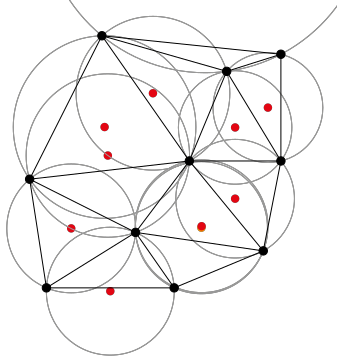
\includegraphics[width=0.5\textwidth]{Circumcircle.png}
  \caption{Illustration of the Delaunay triangulation with all the circumcircles shown \citep{NuEs:2016}.}
  \label{fig:Circumcircle}
\end{figure}

As Arne Laks\aa\, has claimed, GMlib uses it in the background for displaying my objects on the screen, and \cref{alg:DelaunayTriangulation} describes how this triangulation is made. It is based on algorithm described in \citep[Chapter 9.3]{Schwarzkopf1997}.

\begin{algorithm}
  \SetAlgoLined
  \KwData{A set $P$ of $n$ points}
  \KwResult{A Delaunay triangulation of $P$}
  Find the convex hull for the $P$\\
  Make 3 new points (the triangle)\\
  Make 3 new edges and 1 triangle\\
  \For{$\text{each } p \in P$}{
    Find triangle that $p$ is inside of\\
    \uIf{$p$ is inside the triangle}{
      Split the triangle into 3\\
      Check and perform swap if necessary\\
    }
    \Else{
      Split the edge that $p$ lies on in 2 and each triangle into 2\\
      Check and perform swap if necessary\\
    }
  }
  Remove the 3 new points\\
  Remove the edges\\
  \caption{Delanuay triangulation algorithm}
  \label{alg:DelaunayTriangulation}
\end{algorithm}
 
\section{Results \& Discussion} \label{sec:Results}
Result of my project is overall very good, both when it comes to code quality and efficiency. In it I am able to create B-Splines, blend curves, and use them to create GERBS curves and surfaces. \Cref{fig:B-Splines,fig:Blending,fig:GERBSCurve,fig:GERBSSurface} show some of the geometrical objects that my program is capable of rendering.

\begin{figure}[H]
  \centering
  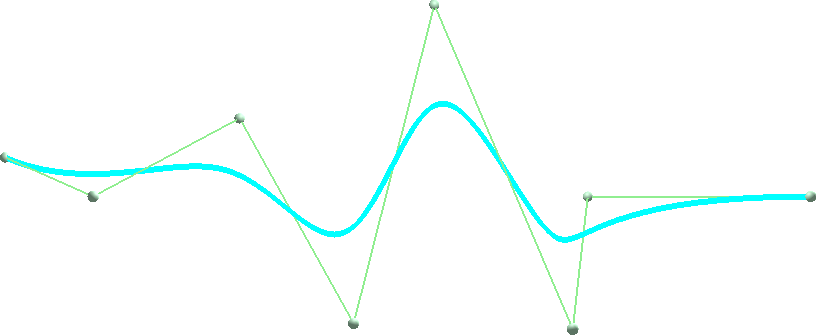
\includegraphics[width=0.49\textwidth]{B-Spline.png}
  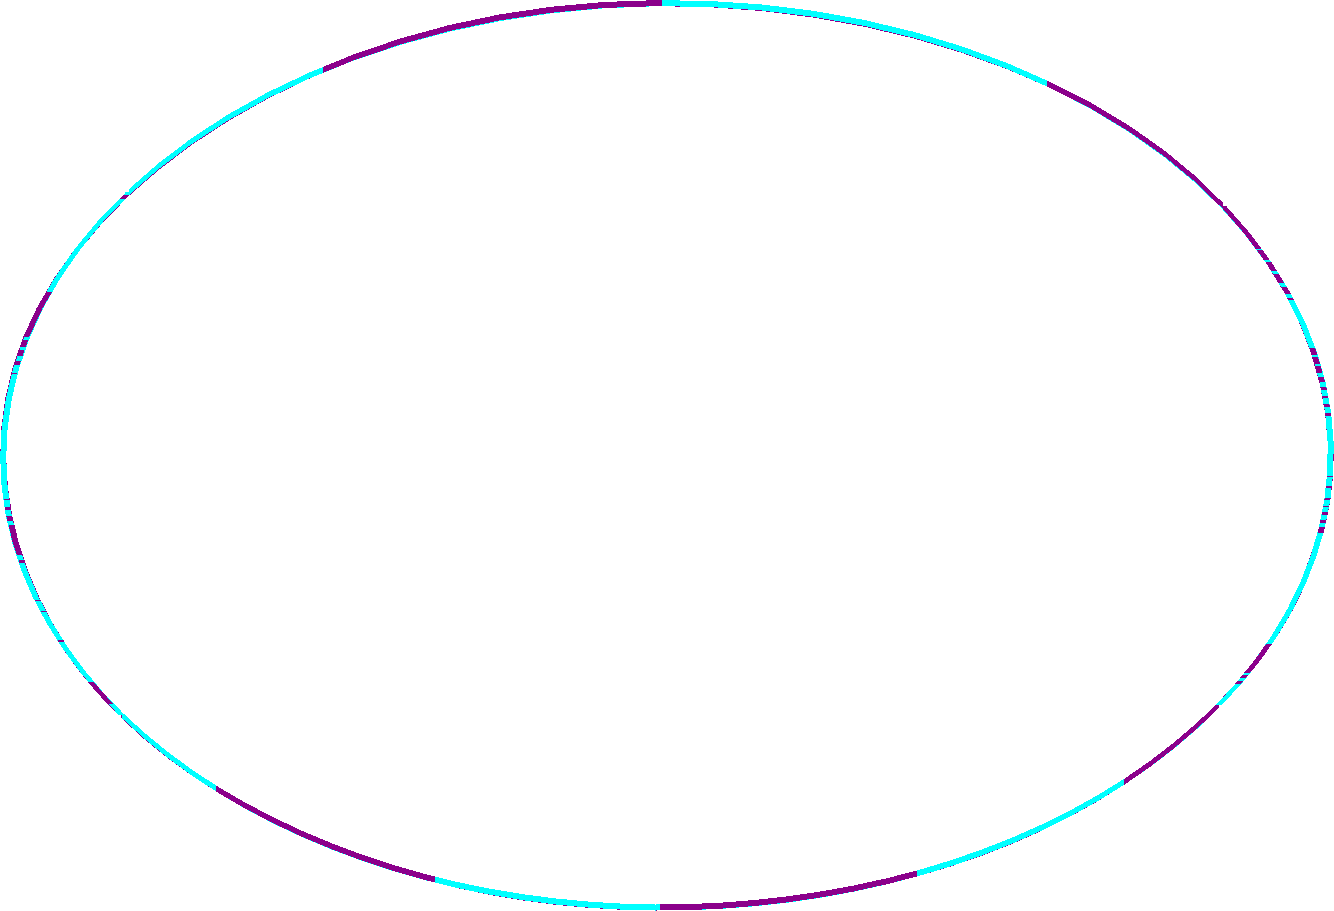
\includegraphics[width=0.49\textwidth]{Sampling.png}
  \caption{Illustration of the B-Splines in my program, one created from a set of control points (left), and one by sampling and least squares method (right).}
  \label{fig:B-Splines}
\end{figure}

\begin{figure}[H]
  \centering
  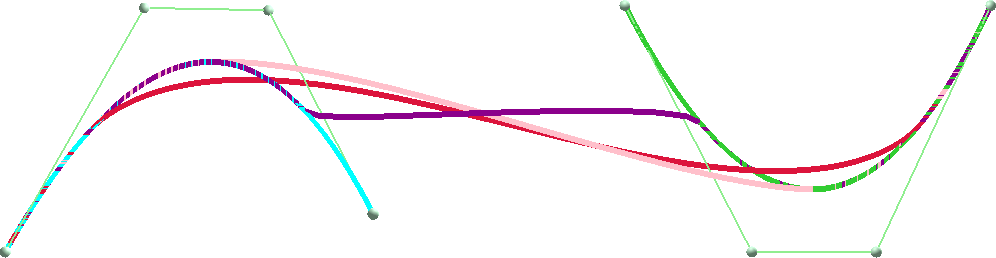
\includegraphics[width=0.8\textwidth]{Blending.png}
  \caption{Illustration of the blending of two curves using 80\% of the original curves (magenta), 50\% (pink), and 20\% (red).}
  \label{fig:Blending}
\end{figure}

\begin{figure}[H]
  \centering
  
\includegraphics[width=0.49\textwidth]{GERBSCurve.png}
  
\includegraphics[width=0.49\textwidth]{LocalCurves.png}
  \caption{Illustration of GERBS curve (left) and its subcurves (right).}
  \label{fig:GERBSCurve}
\end{figure}

\begin{figure}[H]
\centering
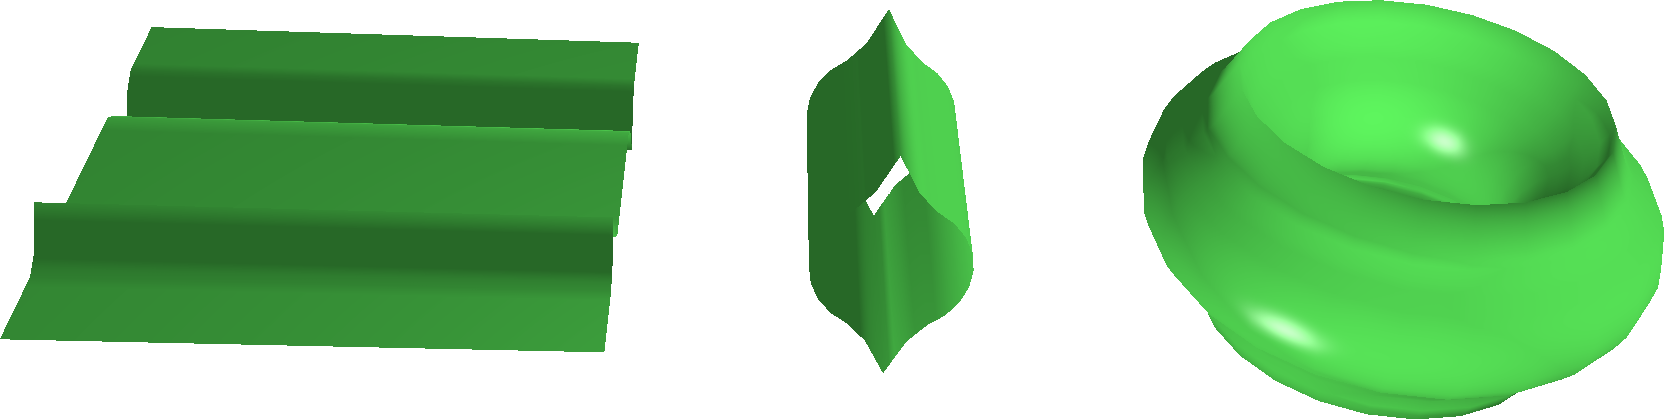
\includegraphics[width=0.8\textwidth]{GERBSSurfaces.png}
\caption{Illustration of GERBS surfaces, a plane, a cylinder, and a torus, with distorted subsurfaces.}
\label{fig:GERBSSurface}
\end{figure}

As it stands my simple B-Splines are static, and are not animated in any way, although adding this functionality is trivial. I chose not to do it to make it easier to show that they are created correctly. And they indeed correspond to tested implementations in GMlib.

Blending curves on the other hand are dynamic, so that changes in any of the two original curves is reflected in the blended curves. The functionality found there makes it easy for me to choose where blending occurs, instead of being limited to a static blending value, presented in \citep[Chapter 6.2.2]{Laksa2012}.

GERBS curve, modeled after curve described by \cref{eq:HeartCurve} is fully dynamic and animated resulting in an animation of a beating heart. This effect is achieved by affine transformations on subcurves. During the animation loop curves 1-4 and 6-9 are translated along $x$-axis whereas curves 0 and 5 are translated along $y$-axis. In addition to that curves 1, 2, 8, and 9 are rotated along two vectors in $xy$-plane. These transformations result in dynamic and smooth animation where heart is stretched in and out.  \Cref{fig:CurveComparison} shows how these translated and rotated curves result in stretched out heart compared to original model curve. It also changes colour of the curve using HSV colour values updated in animation loop.

\begin{figure}[H]
  \centering
  
\includegraphics[width=0.8\textwidth]{CurveComparison.png}
  \caption{Comparison between GERBS curve with transformed local curves (pink), and the model curve (cyan), defined by \cref{eq:HeartCurve}.}
  \label{fig:CurveComparison}
\end{figure}

Affine transformations are a form of a linear mapping method which is used to translate, scale, shear, and rotate objects in affine space. Its properties are: that it preserves \emph{collinearity}, \emph{parallelism}, \emph{convexity}, \emph{barycenters} of points, as well as \emph{ratios of length along a line}. The transformation itself occurs by multiplying objects matrix with the specific matrix for a given transformation. One such matrix, used for translating objects is shown in \cref{eq:TranslationMatrix}, where $x$, $y$, and $z$ specify displacement along their respective axes. And \cref{fig:GERBSCurve} shows how these translated and rotated local curves result in stretched out heart.

\begin{equation}
\begin{bmatrix}
1&0&0&0\\
0&1&0&0\\
0&0&1&0\\
x&y&z&1
\end{bmatrix}
\label{eq:TranslationMatrix}
\end{equation}

Lastly my GERBS surfaces are also working and are displayed correctly. This was tested by creating surfaces for all three cases of closed and open surfaces, inspecting subsurfaces, and performing affine transformations on some of the local subsurfaces. However this is not dynamic as a bug in GMlib's replot function, required to update the surface, causes my program to crash. Therefore I have only transformed the subsurfaces once before the main surface is drawn. However code needed for creating a dynamic animation is implemented, but not activated. If that bug is fixed then I only need to activate this code to get a dynamic animation.

\section{Conclusion}
The main focus of this project was to implement a GERBS curve and animate it, and I have done it quite well. There is nothing that I can complain about how this has been done.

One of the possible further developments might be to extend the functionality of the GERBS curve to work in other dimensions as well as on higher orders.

I am overall very satisfied with both the result of my project and what I have learned about computer graphics and geometry during this course. GERBS curves are not a really well explored subject and most of the papers regarding them talk about practical uses for them, not so much about implementation of them from scratch. I personally think that in a few years time with better computing resources and understanding of them GERBS curves might replace B-Splines as the industry standard or at least become a tempting alternative to them.

Lastly a video showing my program in action can be found here: \url{https://youtu.be/j-YXZdhYR0E}, and repository with my code can be found here: \url{https://source.coderefinery.org/MormonJesus69420/STE6247-Applied-Geometry-And-Special-Effects}.

\section{Acknowledgements}
I would like to thank Christopher Hagerup cha113, Victor Lindb\"{a}ck hli039, Olav Larseng ola014, Kent Larsen kla096, for cooperating on both this report and the project itself.
 
\section{References}
\begingroup
\def\section*#1{}
\bibliographystyle{apalike}
\bibliography{References}
\endgroup
\end{document} 